\documentclass[12pt,letterpaper]{article}
\usepackage[letterpaper,left=.6in,right=.6in,top=.68in,bottom=.65in,headheight=14pt,headsep=14pt,footskip=23pt]{geometry}
\usepackage[T1]{fontenc}
\usepackage{lmodern}
\usepackage{tikz}
\usetikzlibrary{arrows.meta}
\usepackage{fancyhdr}
\pdfmapfile{+lm.map}
\pdfcompresslevel=9
\pdfobjcompresslevel=3
\pagestyle{fancy}
\fancyhf{}
\fancyhead[L]{\fontsize{10.5}{12}\selectfont Week 78 / Three-armed lines / Grades 4--5}
\fancyfoot[L]{\fontsize{9}{11}\selectfont Bellingham Math Circle / Week 78 / F78-S-v3}
\fancyfoot[R]{\fontsize{9}{11}\selectfont\thepage}
\renewcommand{\headrulewidth}{0pt}
\renewcommand{\footrulewidth}{0pt}
\setlength{\parindent}{0pt}
\setlength{\parskip}{6pt}
\renewcommand{\familydefault}{\sfdefault}
\AtBeginDocument{\fontsize{12}{15}\selectfont}
\newcommand{\problem}[2]{\par\noindent\textbf{Problem #1:} #2\par}
\newcommand{\board}[3]{%
\begin{tikzpicture}[x=#1cm,y=#1cm]
 \path[use as bounding box] (-.52,-.52) rectangle (8.42,8.35);
 \draw[step=1,gray!37,line width=.25pt] (0,0) grid (8,8);
 \draw[gray!65,line width=.4pt] (0,0) rectangle (8,8);
 \foreach \v in {0,2,4,6,8}{
   \node[below,font=\fontsize{8}{9}\selectfont] at (\v,0) {\v};
   \node[left,font=\fontsize{8}{9}\selectfont] at (0,\v) {\v};
 }
 #2
 #3
\end{tikzpicture}%
}
\newcommand{\junction}[3]{\fill (#1,#2) circle[radius=2.2pt];\node[above right,xshift=2pt,yshift=2pt,inner sep=2pt,font=\fontsize{10}{12}\selectfont,fill=white,fill opacity=.85,text opacity=1] at (#1,#2) {#3};}
\newcommand{\target}[3]{\draw[line width=.8pt,fill=white] (#1,#2) circle[radius=2.4pt];\node[above right,xshift=2pt,yshift=2pt,inner sep=2pt,font=\fontsize{10}{12}\selectfont,fill=white,fill opacity=.85,text opacity=1] at (#1,#2) {#3};}
\begin{document}
For a point $(x,y)$, compare $x$, $y$, and $2$. When the least number occurs at least twice, the point lies on this line.
\vspace{-2pt}
\begin{center}
\begin{minipage}[c]{.36\linewidth}\centering
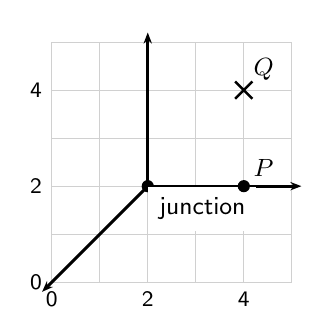
\begin{tikzpicture}[x=.61cm,y=.61cm]
 \path[use as bounding box] (-.5,-.45) rectangle (5.3,5.3);
 \draw[step=1,gray!37,line width=.25pt] (0,0) grid (5,5);
 \foreach \v in {0,2,4}{\node[below,font=\fontsize{8}{9}\selectfont] at (\v,0){\v};\node[left,font=\fontsize{8}{9}\selectfont] at (0,\v){\v};}
 \draw[-{Stealth[length=4pt]},line width=1.1pt] (2,2)--(5.2,2);
 \draw[-{Stealth[length=4pt]},line width=1.1pt] (2,2)--(2,5.2);
 \draw[-{Stealth[length=4pt]},line width=1.1pt] (2,2)--(-.2,-.2);
 \fill (2,2) circle[radius=2.2pt];
 \node[below right,font=\fontsize{9}{11}\selectfont,inner sep=4pt,fill=white] at (2,2){junction};
 \fill (4,2) circle[radius=2.2pt];
 \node[above right,font=\fontsize{9}{11}\selectfont] at (4,2){$P$};
 \draw[line width=.9pt] (3.82,3.82)--(4.18,4.18) (3.82,4.18)--(4.18,3.82);
 \node[above right,font=\fontsize{9}{11}\selectfont] at (4,4){$Q$};
\end{tikzpicture}
\end{minipage}\hfill
\begin{minipage}[c]{.60\linewidth}
$P=(4,2):\quad 4,\ \underline{2},\ \underline{2}$\par
The least number is tied. $P$ is on the line.\par\vspace{5pt}
$Q=(4,4):\quad 4,\ 4,\ \underline{2}$\par
The least number occurs once. $Q$ is off the line.
\end{minipage}
\end{center}
\vspace{-5pt}
The arms point east, north, and diagonally southwest. They continue without end. Every line in this packet has this shape, moved without turning. Points between grid dots count too.

\vspace{10pt}
Here are two completed lines. Blue has junction $U=(1,4)$; orange has junction $V=(4,2)$. Their only shared point is circled: $(4,4)$.
\begin{center}
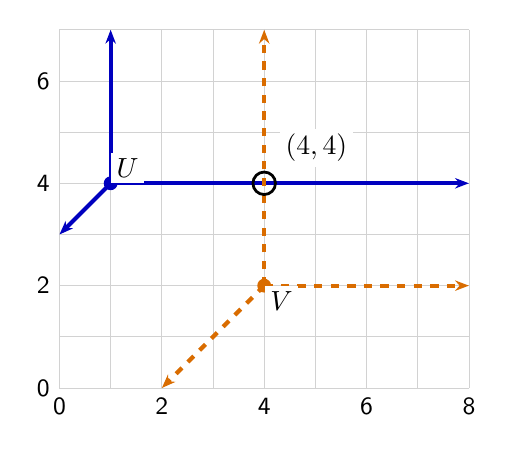
\begin{tikzpicture}[x=.65cm,y=.65cm]
 \draw[step=1,gray!35,line width=.25pt] (0,0) grid (8,7);
 \foreach \v in {0,2,4,6,8}{\node[below,font=\small] at (\v,0){\v};}
 \foreach \v in {0,2,4,6}{\node[left,font=\small] at (0,\v){\v};}
 \draw[blue!75!black,line width=1.5pt,-{Stealth[length=5pt]}] (1,4)--(8,4);
 \draw[blue!75!black,line width=1.5pt,-{Stealth[length=5pt]}] (1,4)--(1,7);
 \draw[blue!75!black,line width=1.5pt,-{Stealth[length=5pt]}] (1,4)--(0,3);
 \draw[orange!85!black,line width=1.5pt,dashed,-{Stealth[length=5pt]}] (4,2)--(8,2);
 \draw[orange!85!black,line width=1.5pt,dashed,-{Stealth[length=5pt]}] (4,2)--(4,7);
 \draw[orange!85!black,line width=1.5pt,dashed,-{Stealth[length=5pt]}] (4,2)--(2,0);
 \fill[blue!75!black] (1,4) circle(2.5pt);\node[above right,fill=white,inner sep=2pt] at (1,4){$U$};
 \fill[orange!85!black] (4,2) circle(2.5pt);\node[below right,fill=white,inner sep=2pt] at (4,2){$V$};
 \draw[black,line width=1pt] (4,4) circle(.22);
 \node[above right,fill=white,inner sep=2pt] at (4.3,4.3){$(4,4)$};
\end{tikzpicture}
\end{center}
In the next problem, try to make two lines share just one point, then try to make two lines overlap along a whole stretch. A shared stretch includes every point between its grid dots.

\newpage

\problem{1}{Choose junction $B$ on each top grid. Make the two lines share just one point on one top grid and a whole stretch on the other. On every grid, draw the lines with junctions $A$ and $B$ in different colours. Circle single shared points and trace the whole shared part heavily.}

\vspace{1pt}

\noindent \board{0.78}{\junction{4}{4}{A}}{}\hfill \board{0.78}{\junction{4}{4}{A}}{}
\par\vspace{7pt}
\noindent \board{0.78}{\junction{2}{2}{A}}{\junction{6}{5}{B}}\hfill \board{0.78}{\junction{2}{2}{A}}{\junction{5}{6}{B}}

\newpage

\problem{2}{Draw the lines with junctions $A$ and $B$ on each grid. Mark every part they share. How many shared points does each pair have?}

\vspace{5pt}

\noindent \board{0.82}{\junction{2}{6}{A}}{\junction{6}{2}{B}}\hfill \board{0.82}{\junction{3}{2}{A}}{\junction{3}{6}{B}}
\par\vspace{7pt}
\noindent \board{0.82}{\junction{2}{4}{A}}{\junction{6}{4}{B}}\hfill \board{0.82}{\junction{2}{2}{A}}{\junction{6}{6}{B}}
\vspace{8pt}

\problem{3}{Can two lines with different junctions share exactly two points? Draw an example, or explain why this cannot happen.}

\vspace{6pt}
\noindent\board{.58}{}{}\hfill\begin{minipage}[b][2.05in][t]{4.3in}\strut\end{minipage}
\vfill

\newpage

\problem{4}{Draw a line through both points on each grid. Its junction may be anywhere, including between grid dots or outside the grid. Can you find a second line through the same two points?}

\vspace{8pt}

\noindent \board{0.83}{\target{2}{6}{P}}{\target{6}{2}{Q}}\hfill \board{0.83}{\target{2}{2}{P}}{\target{6}{5}{Q}}
\vspace{16pt}

\problem{5}{Find all possible junctions of a line through each pair of points.}

\vspace{9pt}

\noindent \board{0.66}{\target{2}{4}{P}}{\target{6}{4}{Q}}\hfill \board{0.66}{\target{3}{2}{P}}{\target{3}{6}{Q}}\hfill \board{0.66}{\target{2}{2}{P}}{\target{5}{5}{Q}}

\vfill

\newpage

\problem{6}{Find where the lines with junctions $A=(2,7)$ and $B=(10,5)$ \ meet. Can any two lines miss each other? Explain your answer. Give a rule for when two lines share more than one point. Your rule must also work for junctions between grid dots or outside this page.}

\vspace{8pt}

\noindent \board{0.76}{\junction{2}{7}{A}}{}
\hfill\begin{minipage}[b][2.65in][t]{3.7in}\strut\end{minipage}
\vspace{14pt}

\problem{7}{Find a rule that tells how many lines can pass through two different points. Explain why your rule works.}

\vspace{8pt}
\noindent\board{.76}{}{}\hfill\begin{minipage}[b][2.65in][t]{3.7in}\strut\end{minipage}
\vfill
\end{document}
